\documentclass[12pt]{scrartcl}

 

\usepackage[utf8]{inputenc}

\usepackage[T1]{fontenc}

\usepackage{lmodern}

\usepackage[ngerman]{babel}

\usepackage{amsmath}

\usepackage{graphicx}


 

\title{Versuch E3\\ Elektronen im elektrischen und magnetischen Feld}

\author{Frederik Strothmann, Henrik Jürgens}

\date{\today}


\begin{document}


 %deckblatt erstellen

\maketitle
\tableofcontents
\newpage

%einleitung zu dem experiment

\section{Einleitung}
Mit Hilfe einer Oszillographenröhre soll die Bewegung von Elektronen unter dem Einfluß äußerer Felder untersucht werden. Dazu beschäftigen wir uns zunächst mit dem Grundprinzip eines Oszillographen, der Ablenkung von Elektronenstrahlen durch elektrische Felder. Ebenso können Elektronenstrahlen durch magnetische Felder abgelenkt werden, hierzu verwenden wir das Magnetfeld eines Helmholtz-Spulenpaares. Zum Schluß versuchen wir, mit diesem Effekt Richtung und Größe des Erdmagnetfeldes zu bestimmen.

%versuchsaufbau mit skizze

\section{Versuchsaufbau}
Der Versuchsaufbau besteht aus einer Oszillographenröhre, einem Steuerkasten, einer Helmholtz-Spule und einem Auffangschirm.
Der Steuerkasten wird an die Oszillographenröhre angeschlossen, um verschiedene Spannungen zu kontrollieren. Dahinter befindet sich die Helmholtz-Spule um im zweiten Aufbau ein Magnetfeld zu erzeugen. Am Ende des Aufbaus befindet sich der Auffangschirm, an welchem die Elektronen detektiert werden.

\begin{figure}[htbp] 
  \centering
    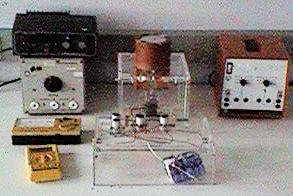
\includegraphics[scale = 0.5]{aufbau.JPG}
  	\caption[Foto der Hauptbestandteile des Versuchs]{Foto der Hauptbestandteile des Versuchs\footnotemark}
  \label{fig:aufbau}
\end{figure}
\footnotetext{Graphik wurde am 22.08.2014 von der Seite: http://www.atlas.uni-wuppertal.de/~kind/apjpg/ap1e3a.JPG entnommen}

\section{Versuchsdurchführung}


\subsection{Praktische Durchführung}

\begin{itemize}
\item	l$_{12}$:	Länge der ersten Ablenkplatten
\item	L$_{12}$:	Abstand zwischen dem Ende der Ablenkplatten bis zum Auffangschirm
\item	d$_{12}$:	Abstand zwischen den ersten Ablenkplatten
\item	l$_{34}$:	Länge der zweiten Ablenkplatten
\item	L$_{34}$:	Abstand zwischen dem Ende der Ablenkplatten bis zum Auffangschirm
\item	d$_{34}$:	Abstand zwischen den zweiten Ablenkplatten
\end{itemize}


\begin{itemize}
\item[(a)] Ablenkung im transversalen elektrischen Feld
\newline
\begin{enumerate}
\item
Messen Sie mit einem Lineal an einer Musterröhre die Abstände
L$_{12}$, l$_{12}$ und d$_{12}$
sowie L$_{34}$, l$_{34}$ und d$_{34}$ für die beiden Ablenkplattenpaare. Als Richtwerte können Sie annehmen:
l$_{12}$ = l$_{34}$ = 35$\pm$2mm. Es steht eine geöffnete Röhre zur Verfügung,
an der Sie L$_{12}$ und L$_{34}$ abschätzen können.
Da die Ablenkplatten teilweise gebogen sind (siehe Abbildung der Röhre im An-
hang), müssen Sie für den Meßwert des Plattenabstands
d$_{12}$ und d$_{34}$ eine vernünftige Abschätzung machen. Ein Wert zwischen 2 und 5 mm sollte sinnvoll sein.
\begin{figure}[htbp] 
	  \centering
	    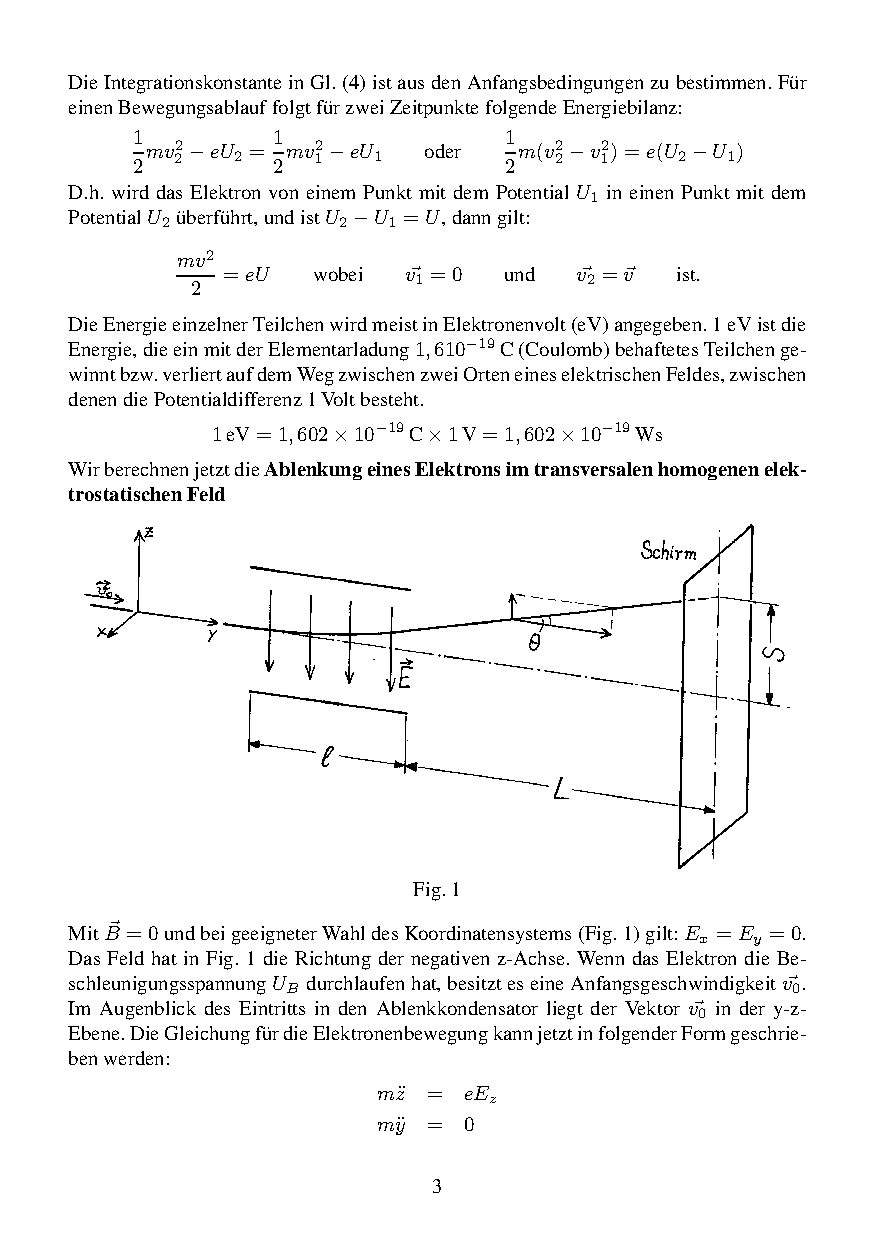
\includegraphics[trim = 1mm 61mm 1mm 85mm, clip, scale = 1]{E_ablenkung.pdf}
	  	\caption[Skizze für die Ablenkung der Elektronen durch das E-Feld]{Skizze für die Ablenkung der Elektronen durch das E-Feld\footnotemark}
	  \label{fig:E_ablenkung}
	\end{figure}
	\footnotetext{Abbildung entnommen von http://www.atlas.uni-wuppertal.de/~kind/E3.pdf Seite 3 am 22.08.2014}
\item
Setzen Sie die Oszillographenröhre mit Hilfe des Schaltplans in 
\begin{figure}[htbp] 
	  \centering
	    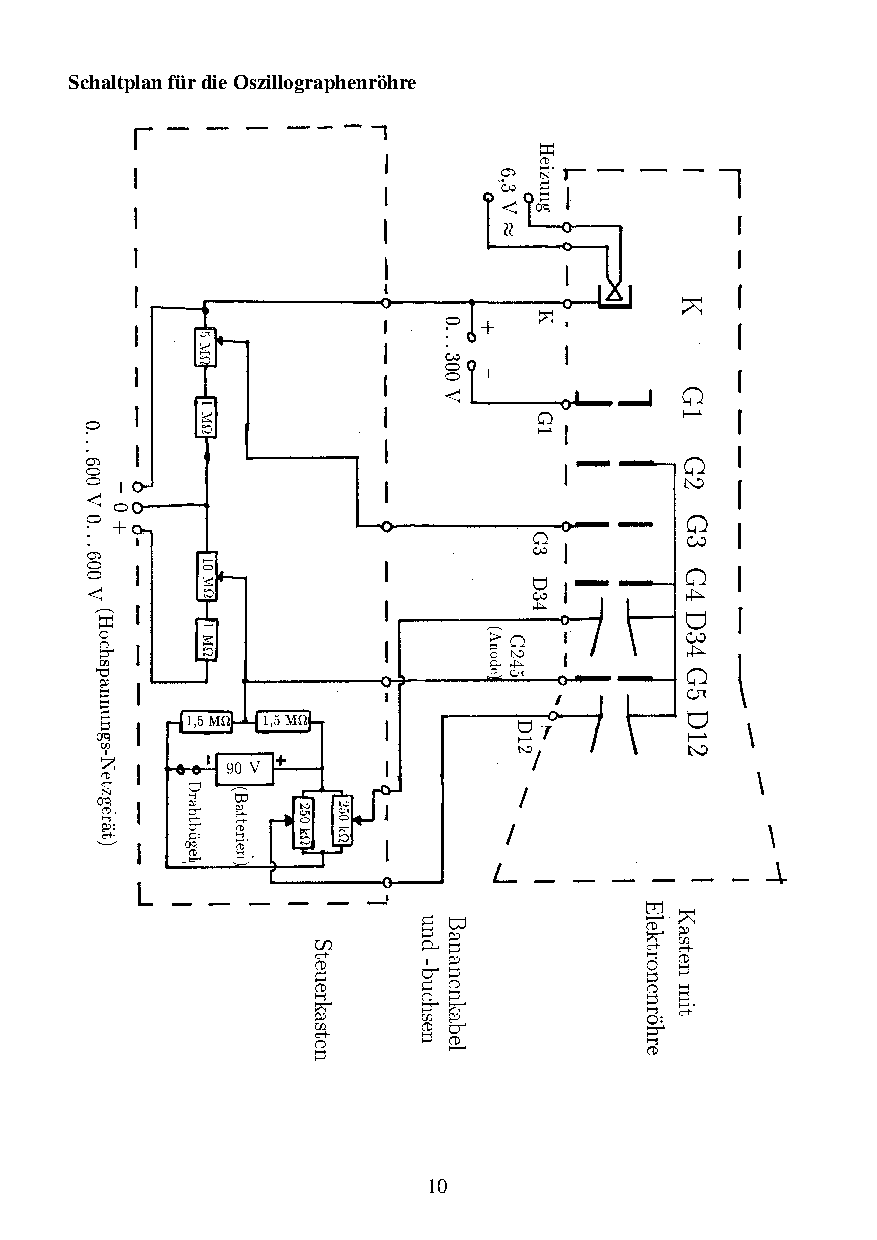
\includegraphics[trim = 1mm 17mm 1mm 17mm, clip, scale = 0.5, angle =90]{schaltskizze.pdf}
	  	\caption[Schaltskizze der Oszillographenröhre und den Schaltkasten]{Schaltskizze der Oszillographenröhre und den Schaltkasten\footnotemark}
	  \label{fig:schaltskizze}
	\end{figure}
	\newpage
	\footnotetext{Abbildung entnommen von http://www.atlas.uni-wuppertal.de/~kind/E3.pdf Seite 10 am 22.08.2014}
Betrieb und stellen Sie einen scharfen Leuchtfleck ein (U$_{D12}$ = U$_{D34}$ = 0, d.h. verbinden Sie die Anschlüsse D12 und D34 mit G245).
\item
Messen Sie für eine feste Beschleunigungsspannung U$_{B}$
die Ablenkung S$_{12}$ als
Funktion der Ablenkspannung U$_{D12}$. Tragen Sie S$_{12}$
als Funktion von U$_{D12}$ in einem Diagramm auf.
\item
Wiederholen Sie diese Messung und die graphische Darstellung mit den Ablenkplatten D34.
\item
Ändern Sie die Beschleunigungsspannung U$_B$, optimieren Sie die Fokussierung
und wiederholen Sie die Messungen 3 und 4 für zwei weitere Werte von U$_B$. Stellen Sie auch diese vier Messungen graphisch dar.
\item
Als graphische Darstellung dieser 6 Messungen aus
3, 4 und 5 erwarten Sie Ursprungsgeraden, z.B. S$_{12}$ = k$_{12}$· U$_{D12}$ (warum? Welche Ursache könnte es
haben, wenn sich keine exakte Ursprungsgerade ergibt?)
Bestimmen Sie die drei Steigungen k$_{12}$ und die drei Steigungen k$_{34}$.
Berechnen Sie für alle 6 Steigungen das Produkt U$_B\cdot$k
mit der entsprechenden
Beschleunigungsspannung. Die drei Produkte U$_B\cdot$k$_{12}$
sollten etwa gleich sein
(warum?), ebenso die drei Produkte U$_B\cdot$k$_{34}$.
\item
Berechnen Sie den Mittelwert der drei Produkte U$_B\cdot$k$_{12}$. Aus diesem Mittelwert können Sie mit den gemessenen L$_{12}$ und l$_{12}$ den Plattenabstand d$_{12}$ bestimmen (nach welcher Formel?). Vergleichen Sie den so erhaltenen Wert mit dem der direkten Messung von d$_{12}$ an der Röhre.
\item
Bestimmen Sie ebenso aus dem Mittelwert der drei Produkte U$_B\cdot$k$_{34}$ und den
gemessenen L$_{34}$ und l$_{34}$ den Plattenabstand d$_{34}$. Vergleichen Sie auch diesen Wert mit dem der direkten Messung von d$_{34}$.
\item
Diskutieren Sie die Fehler, mit denen Ihre Messungen behaftet sind.
\end{enumerate}
\item[(b)] Ablenkung im transversalen Magnetfeld
\newline

\begin{figure}[htbp] 
  \centering
    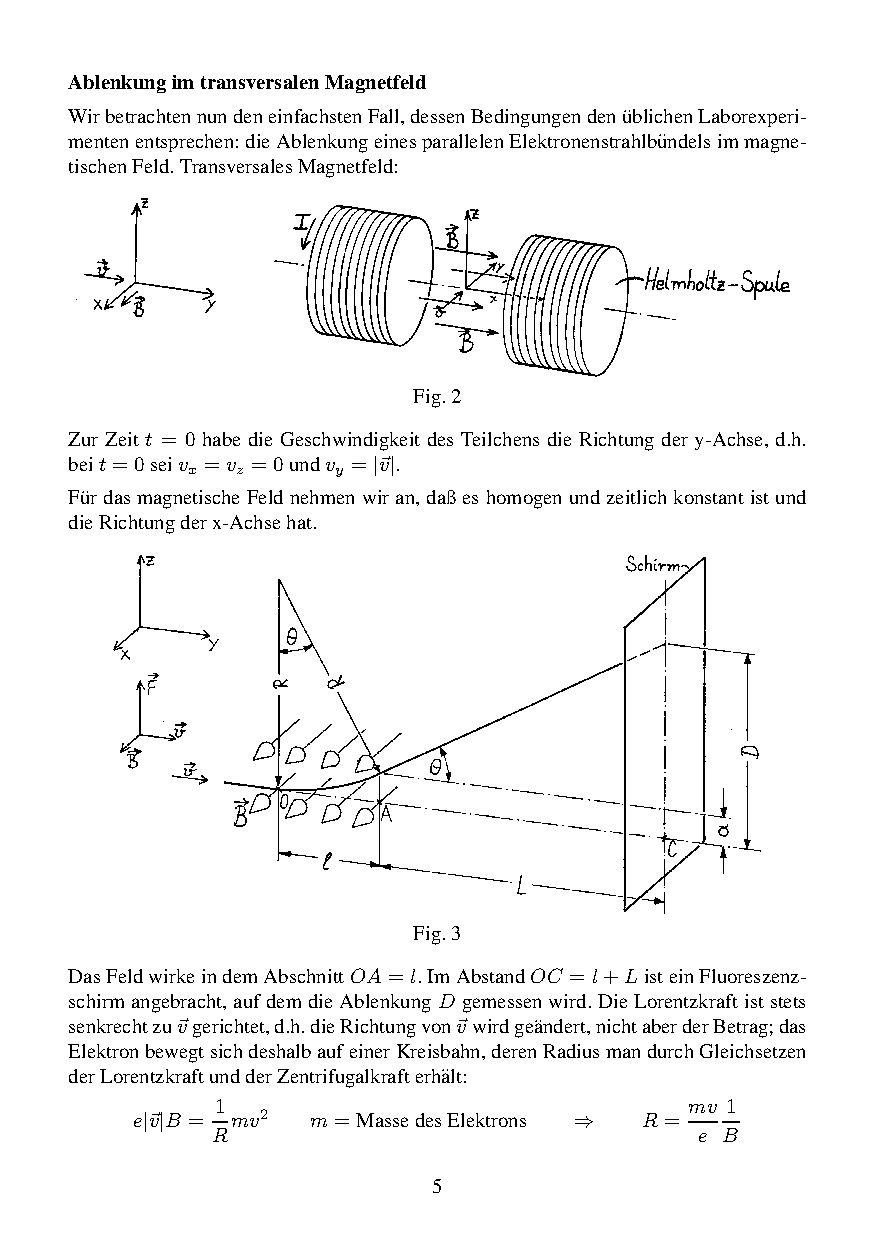
\includegraphics[trim = 1mm 55mm 1mm 91mm, clip, scale = 1]{B_ablenkung.pdf}
  	\caption[Skizze für die Ablenkung der Elektronen durch das B-Feld]{Skizze für die Ablenkung der Elektronen durch das B-Feld\footnotemark}
  \label{fig:E_ablenkung}
\end{figure}
\footnotetext{Abbildung entnommen von http://www.atlas.uni-wuppertal.de/~kind/E3.pdf Seite 5 am 22.08.2014}
Im Folgenden wird anstatt D auch S$_S$ verwendet	
\begin{enumerate}
\item[10.]
Die Röhre wird betrieben wie in (a). Die Ablenkplatten werden nicht benutzt, werden aber an die Anode (G245) angeschlossen. So wird eine statische Aufladung der Platten verhindert, die eine ungewollte Ablenkung zur Folge haben kann. Da Sie im weiteren Verlauf des Versuchs keine Ablenkspannungen
U$_{12}$ und U$_{34}$ mehr benötigen, schalten Sie bitte den 90-V-Batterieblock ab (entfernen sie den Drahtbügel
an der Seite des Steuerkastens.) Die beiden Spulen sind in Serie geschaltet, so daß sich die beiden Magnetfelder addieren. Gemessen wird die an den Spulen angelegte Spannung U$_S$. Sie ist proportional zum Strom, der durch die Spulen fließt, und damit proportional zum Magnetfeld.
\item[11.]
Messen Sie die Strahlablenkung S$_S$ als Funktion der Spulenspannung U$_S$ für feste
Beschleunigungsspannung U$_B$
und stellen Sie die Messung graphisch dar.
\item[12.]
Wiederholen Sie die Messung und graphische Darstellung für zwei andere Beschleunigungsspannungen.
\item[13.]
Sie erwarten Ursprungsgeraden S$_S$ = k$_S\cdot$U$_S$ (wieso?). Bestimmen Sie die drei Steigungen k$_S$. Berechnen Sie für jedes k$_S$
das entsprechende Produkt k$_S\cdot\sqrt{U_\text{B}}$. Vergleichen Sie
diese drei Produkte miteinander. Was erwarten Sie (warum?)
.
\end{enumerate}
\item[(c)] Erdmagnetfeld
\newline
\begin{enumerate}
\item[14.]
In (a) und (b) haben Sie beobachtet, daß bei Abwesenheit von ablenkenden Feldern die Lage des Punktes sich ändert, wenn die Beschleunigungsspannung geändert wird. Ein Grund für diesen Effekt ist das Erdmagnetfeld. Versuchen Sie, durch Markierung mit einem Fettstift auf dem Schirm eine Orientierung der Röhre zu finden, für die keine Ablenkung auftritt. Wie ist in dieser Lage die Beziehung zwischen Achsenrichtung (Elektronenstrahl) und Richtung des Magnetfeldes der Erde?
\item[15.]
Versuchen Sie jetzt, eine Orientierung zu finden, für die die Ablenkung ein Maximum hat. Bestimmen Sie die Richtung und Stärke des Magnetfeldes. Beachten Sie, daß in diesem Fall l die gesamte Länge zwischen Anode und dem Schirm ist und L = 0. Die Elektroden der jetzt verwendeten Röhren sind teilweise aus unmagnetischem Material. Für l
sollten Sie daher die Strecke mindestens von G4 zum Schirm
ansetzen (bei ferromagnetischen Ablenkplatten würde der Strahl magnetisch abgeschirmt und für l wäre der Abstand von G5 zum Schirm anzusetzen). Vergleichen Sie Ihre Bestimmung von Größe und Richtung des Erdmagnetfeldes mit Literaturwerten.
\end{enumerate}

\end{itemize}

\subsection{Theoretische Durchführung}
\begin{itemize}
\item[6.]
Der Fehler von $U \cdot k$ ist:
\begin{align}
\sigma_U = \sqrt{\left(U \sigma_k \right)^2+\left(k \sigma_U\right)^2}
\end{align}
\item[7.]
Der Mittelwert ist:
\begin{align}
M = \frac{(U_{\text{B}}k)_1+
(U_{\text{B}}k)_2+
(U_{\text{B}}k)_3}{3}
\label{eqn:mittel}
\end{align}
Der Fehler auf den Mittelwert ist:
\begin{align}
\sigma_M =\sqrt{
\left(\frac{\sigma_{(U_{\text{B}}k)_1}}{3}\right)^2+ \left(\frac{\sigma_{(U_{\text{B}}k)_2}}{3}\right)^2+
\left(\frac{\sigma_{(U_{\text{B}}k)_3}}{3}\right)^2}
\label{eqn:mittel_sigma}
\end{align}
Der Plattenabstand d berechnet sich nach der Formel:
\begin{align}
d= \frac{L l}{2 U_\text{B} k}
\label{eqn:Plattenabstand}
\end{align}
(wobei $\tan(\theta) \simeq \frac{S}{L}$ nur für $L \gg S$ gilt.)\\
Mit dem Fehler:
\begin{align}
\sigma_d = \sqrt{
\left(\frac{l}{2 U_\text{B} k}\sigma_{L}\right)^2+
\left(\frac{L}{2 U_\text{B} k}\sigma_l\right)^2+
\left(\frac{L l}{2 (U_\text{B} k)^2}\sigma_{U_\text{B} k}\right)^2}
\label{eqn:Plattenabstand_sigma}
\end{align}
\item[8.]
Berechung der Werte analog zu 7.
\item[13.]
Da die magnetische Flussdichte proportional zur Spulenspannung U$_S$ und k die Steigung der Geraden vom Plot von U$_S$ gegen S$_S$ ist, erwarten wir, dass das Produkt $k\cdot\sqrt{U_B}$ nach folgender Formel konstant ist:
\begin{align}
S_S = \frac{leB}{\sqrt{2em U_B}}(L+\frac{1}{2}l)
\label{eqn:AuslenkungSpulenspannung}
\end{align}
Diese Formel gilt jedoch nur für kleine Auslenkwinkel $\theta$
Der Fehler von $\sqrt{U_\text{B}} \cdot k$ ist:
\begin{align}
\sigma_{\sqrt{U_\text{B}}k} = \sqrt{
\left(\frac{k}{2\sqrt{U_\text{B}}}\sigma_{U_\text{B}}\right)^2+
\left(\sqrt{U_\text{B}}\sigma{k}\right)^2}
\label{eqn:AuslenkungSpulenspannung_sigma}
\end{align}
\item[15.]
Die Formel zur Berechnung des B-Feldes ist:
\begin{align}
B = \frac{2 S_\text{S}\sqrt{2 m_e U_\text{B}}}{l^2 \sqrt{e}}
\label{eqn:bfeld}
\end{align}
Mit einem Fehler von:
\begin{align}
\sigma_B = \sqrt{
\left(\frac{2 \sqrt{2 m_e U_\text{B}}}{l^2 \sqrt{e}}\sigma_{S_\text{S}}\right)^2+
\left(\frac{S_\text{S}\sqrt{2 m_e}}{l^2 \sqrt{e U_\text{B}}}\sigma{U_\text{B}}\right)^2+
\left(\frac{4 S_\text{S}\sqrt{2 m_e U_\text{B}}}{l^3 \sqrt{e}}\sigma_l\right)^2
}
\label{eqn:bfeld_sigma}
\end{align}
\end{itemize}

\section{Messergebnisse}

\begin{table}[htbp]
\caption{Abstände der einzelnen Komponenten}
\begin{center}
\begin{tabular}{|l|r|r|l|r|r|}
\hline
Bezeichnung & \multicolumn{1}{l|}{Längen/mm} & \multicolumn{1}{l|}{Fehler/mm} & Bezeichnung & \multicolumn{1}{l|}{Längen/mm} & \multicolumn{1}{l|}{Fehler/mm} \\ \hline
L\_12 & 75 & 3 & L\_34 & 113 & 3 \\ \hline
l\_12 & 35 & 2 & l\_34 & 35 & 2 \\ \hline
d\_12 & 3,5 & 1,5 & d\_34 & 3,5 & 1,5 \\ \hline
\end{tabular}
\end{center}
\label{tab:materialeigenschaften}
\end{table}

\newpage

\subsection{elektrisches Feld}
\subsubsection{X-Achsenauslenkung}



\begin{table}[htbp]
\caption{Daten der Messung für eine Beschleunigungsspannung von 1130V}
\begin{center}
\begin{tabular}{|r|r|r|r|}
\hline
\multicolumn{1}{|l|}{S\_12/mm} & \multicolumn{1}{l|}{Fehler/mm} & \multicolumn{1}{l|}{U\_D\_12/V} & \multicolumn{1}{l|}{Fehler/V} \\ \hline
-5,8 & 0,2 & -20 & 0,06 \\ \hline
-3,6 & 0,2 & -12 & 0,06 \\ \hline
-2,4 & 0,2 & -8 & 0,06 \\ \hline
-1,2 & 0,2 & -4 & 0,06 \\ \hline
0 & 0,2 & 0 & 0,06 \\ \hline
1,4 & 0,2 & 5 & 0,06 \\ \hline
3 & 0,2 & 10 & 0,06 \\ \hline
4,3 & 0,2 & 15 & 0,06 \\ \hline
5,7 & 0,2 & 20 & 0,06 \\ \hline
\end{tabular}
\end{center}
\label{tab:materialeigenschaften}
\end{table}



\begin{table}[htbp]
\caption{Daten der Messung für eine Beschleunigungsspannung von 1350V}
\begin{center}
\begin{tabular}{|r|r|r|r|}
\hline
\multicolumn{1}{|l|}{S\_12/mm} & \multicolumn{1}{l|}{Fehler/mm} & \multicolumn{1}{l|}{U\_D\_12/V} & \multicolumn{1}{l|}{Fehler/V} \\ \hline
-4,9 & 0,2 & -20 & 0,06 \\ \hline
-2,5 & 0,2 & -10 & 0,06 \\ \hline
0 & 0,2 & 0 & 0,06 \\ \hline
2,5 & 0,2 & 10 & 0,06 \\ \hline
4,9 & 0,2 & 20 & 0,06 \\ \hline
\end{tabular}
\end{center}
\label{tab:materialeigenschaften}
\end{table}




\begin{table}[htbp]
\caption{Daten der Messung für eine Beschleunigungsspannung von 475V}
\begin{center}
\begin{tabular}{|r|r|r|r|}
\hline
\multicolumn{1}{|l|}{S\_12/mm} & \multicolumn{1}{l|}{Fehler/mm} & \multicolumn{1}{l|}{U\_D\_12/V} & \multicolumn{1}{l|}{Fehler/V} \\ \hline
-14,8 & 0,2 & -20 & 0,06 \\ \hline
-7,6 & 0,2 & -10 & 0,06 \\ \hline
0 & 0,2 & 0 & 0,06 \\ \hline
7 & 0,2 & 10 & 0,06 \\ \hline
14,3 & 0,2 & 20 & 0,06 \\ \hline
\end{tabular}
\end{center}
\label{tab:materialeigenschaften}
\end{table}

\newpage

\subsubsection{Y-Achsenauslenkung}


\begin{table}[htbp]
\caption{Daten der Messung für eine Beschleunigungsspannung von 1130V}
\begin{center}
\begin{tabular}{|r|r|r|r|}
\hline
\multicolumn{1}{|l|}{S\_12/mm} & \multicolumn{1}{l|}{Fehler/mm} & \multicolumn{1}{l|}{U\_D\_12/V} & \multicolumn{1}{l|}{Fehler/V} \\ \hline
-14,8 & 0,2 & -20 & 0,06 \\ \hline
-11,3 & 0,2 & -15 & 0,06 \\ \hline
-7,5 & 0,2 & -10 & 0,06 \\ \hline
-3,85 & 0,2 & -5 & 0,06 \\ \hline
0 & 0,2 & 0 & 0,06 \\ \hline
3,8 & 0,2 & 5 & 0,06 \\ \hline
7,7 & 0,2 & 10 & 0,06 \\ \hline
11,6 & 0,2 & 15 & 0,06 \\ \hline
15 & 0,2 & 20 & 0,06 \\ \hline
\end{tabular}
\end{center}
\label{tab:materialeigenschaften}
\end{table}



\begin{table}[htbp]
\caption{Daten der Messung für eine Beschleunigungsspannung von 1150V}
\begin{center}
\begin{tabular}{|r|r|r|r|}
\hline
\multicolumn{1}{|l|}{S\_12/mm} & \multicolumn{1}{l|}{Fehler/mm} & \multicolumn{1}{l|}{U\_D\_12/V} & \multicolumn{1}{l|}{Fehler/V} \\ \hline
-15,1 & 0,2 & -20 & 0,06 \\ \hline
-11,1 & 0,2 & -15 & 0,06 \\ \hline
-7,5 & 0,2 & -10 & 0,06 \\ \hline
-3,9 & 0,2 & -5 & 0,06 \\ \hline
0 & 0,2 & 0 & 0,06 \\ \hline
3,9 & 0,2 & 5 & 0,06 \\ \hline
7,9 & 0,2 & 10 & 0,06 \\ \hline
12,2 & 0,2 & 15 & 0,06 \\ \hline
16 & 0,2 & 20 & 0,06 \\ \hline
\end{tabular}
\end{center}
\label{tab:materialeigenschaften}
\end{table}




\begin{table}[htbp]
\caption{Daten der Messung für eine Beschleunigungsspannung von 1325V}
\begin{center}
\begin{tabular}{|r|r|r|r|}
\hline
\multicolumn{1}{|l|}{S\_12/mm} & \multicolumn{1}{l|}{Fehler/mm} & \multicolumn{1}{l|}{U\_D\_12/V} & \multicolumn{1}{l|}{Fehler/V} \\ \hline
-12,9 & 0,2 & -20 & 0,06 \\ \hline
-9,8 & 0,2 & -15 & 0,06 \\ \hline
-6,45 & 0,2 & -10 & 0,06 \\ \hline
-2,8 & 0,2 & -5 & 0,06 \\ \hline
0 & 0,2 & 0 & 0,06 \\ \hline
3 & 0,2 & 5 & 0,06 \\ \hline
6,5 & 0,2 & 10 & 0,06 \\ \hline
10,1 & 0,2 & 15 & 0,06 \\ \hline
13,6 & 0,2 & 20 & 0,06 \\ \hline
\end{tabular}
\end{center}
\label{tab:materialeigenschaften}
\end{table}

\newpage

\subsection{magnetisches Feld}


\begin{table}[htbp]
\caption{Daten der Messung für eine Beschleunigungsspannung von 1100V}
\begin{center}
\begin{tabular}{|r|r|r|r|}
\hline
\multicolumn{1}{|l|}{S\_12/mm} & \multicolumn{1}{l|}{Fehler/mm} & \multicolumn{1}{l|}{U\_S/V} & \multicolumn{1}{l|}{Fehler/V} \\ \hline
0 & 0,4 & 0 & 0,006 \\ \hline
3,5 & 0,4 & 0,5 & 0,006 \\ \hline
6 & 0,4 & 1 & 0,006 \\ \hline
9,7 & 0,4 & 1,5 & 0,006 \\ \hline
13,1 & 0,4 & 2 & 0,006 \\ \hline
\end{tabular}
\end{center}
\label{tab:materialeigenschaften}
\end{table}


\begin{table}[htbp]
\caption{Daten der Messung für eine Beschleunigungsspannung von 1180V}
\begin{center}
\begin{tabular}{|r|r|r|r|}
\hline
\multicolumn{1}{|l|}{S\_12/mm} & \multicolumn{1}{l|}{Fehler/mm} & \multicolumn{1}{l|}{U\_S/V} & \multicolumn{1}{l|}{Fehler/V} \\ \hline
0 & 0,4 & 0 & 0,006 \\ \hline
6,1 & 0,4 & 1 & 0,006 \\ \hline
8,5 & 0,4 & 1,5 & 0,006 \\ \hline
12,2 & 0,4 & 2 & 0,006 \\ \hline
16,9 & 0,4 & 3 & 0,006 \\ \hline
\end{tabular}
\end{center}
\label{tab:materialeigenschaften}
\end{table}


\begin{table}[htbp]
\caption{Daten der Messung für eine Beschleunigungsspannung von 350V}
\begin{center}
\begin{tabular}{|r|r|r|r|}
\hline
\multicolumn{1}{|l|}{S\_12/mm} & \multicolumn{1}{l|}{Fehler/mm} & \multicolumn{1}{l|}{U\_S/V} & \multicolumn{1}{l|}{Fehler/V} \\ \hline
0 & 0,4 & 0 & 0,006 \\ \hline
3,8 & 0,4 & 0,3 & 0,006 \\ \hline
7 & 0,4 & 0,5 & 0,006 \\ \hline
9,4 & 0,4 & 0,7 & 0,006 \\ \hline
12,4 & 0,4 & 1 & 0,006 \\ \hline
\end{tabular}
\end{center}
\label{tab:materialeigenschaften}
\end{table}

\newpage

\section{Auswertung}
\subsection{elektrisches Feld}
Für die Ablenkung der Kathodenstrahlen entlang der X-Achse ergaben sich die folgenden Plots:\\
Für eine Beschleunigungsspannung von 1130V ergab sich die Regressionsgerade mit f(x)=$0,290 (\pm 0,002 ) x  - 0,038 (\pm 0,02)$, mit einem $\chi^2$ von 0,122845.


\begin{figure}[htbp] 
  \centering
    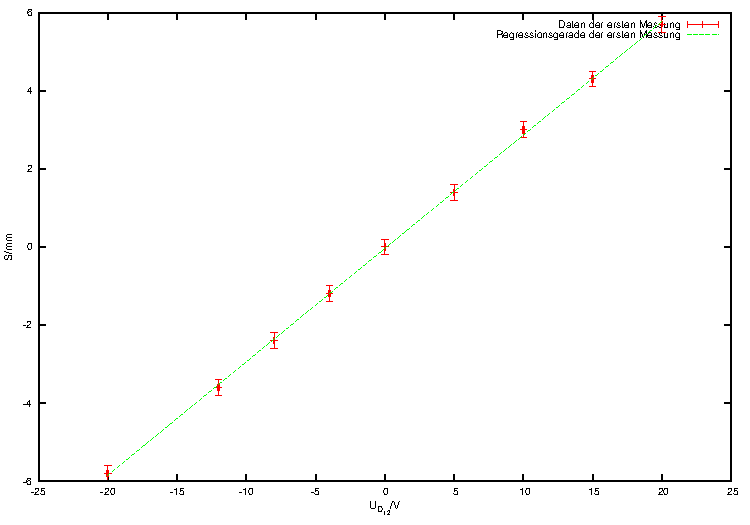
\includegraphics[scale = 1]{x_1.pdf}
  	\caption[Plot der Auslenkung in Abhängigkeit der Ablenkungsspannung, bei 1130V Beschleunigungsspannung]{Plot der Auslenkung in Abhängigkeit der Ablenkungsspannung, bei 1130V Beschleunigungsspannung}
  \label{fig:x_1}
\end{figure}



\newpage

Für eine Beschleunigungsspannung von 1350V ergab sich die Regressionsgerade mit f(x)=$0,246 (\pm 0,001) x  + 2,13E-013	 (\pm 0,01)$, mit einem $\chi^2$ von $0,0\overline{3}$. %0,0333333 stand vorher da


\begin{figure}[htbp] 
  \centering
    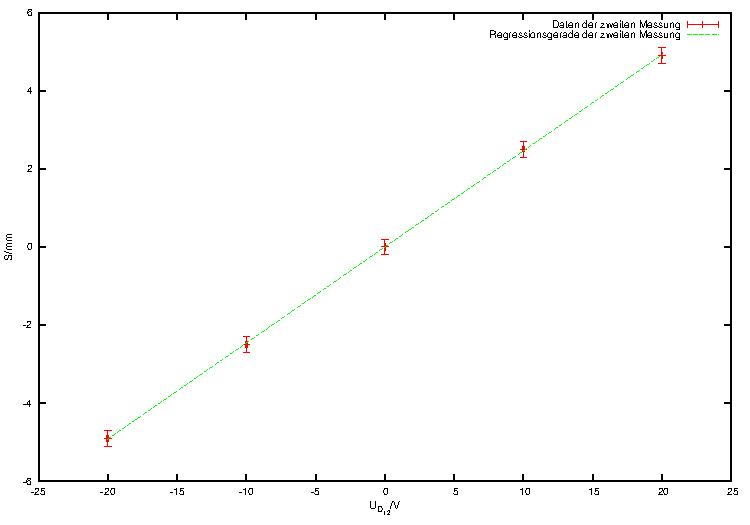
\includegraphics[scale = 1]{x_2.pdf}
  	\caption[Plot der Auslenkung in Abhängigkeit der Ablenkungsspannung, bei 1350V Beschleunigungsspannung]{Plot der Auslenkung in Abhängigkeit der Ablenkungsspannung, bei 1350V Beschleunigungsspannung}
  \label{fig:x_1}
\end{figure}



\newpage

Für eine Beschleunigungsspannung von 475V ergab sich die Regressionsgerade mit f(x)=$0,728 (\pm 0,005) x - 0,22 (\pm 0,07)$, mit einem $\chi^2$ von $0,5\overline{3}$.
%0.533333 stand vorher da

\begin{figure}[htbp] 
  \centering
    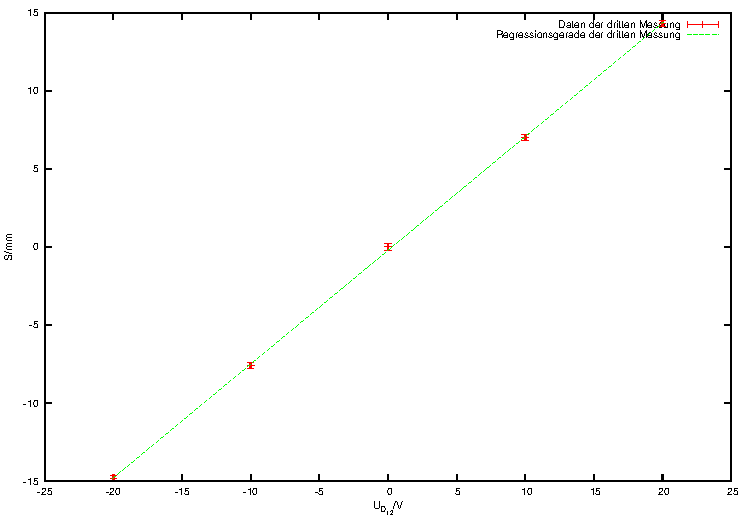
\includegraphics[scale = 1]{x_3.pdf}
  	\caption[Plot der Auslenkung in Abhängigkeit der Ablenkungsspannung, bei 475V Beschleunigungsspannung]{Plot der Auslenkung in Abhängigkeit der Ablenkungsspannung, bei 475V Beschleunigungsspannung}
  \label{fig:x_1}
\end{figure}




\newpage

Für die Auslenkung in Y-Achsenrichtung ergaben sich die folgenden Plots:

Für eine Beschleunigungsspannung von 1130V ergab sich die Regressionsgerade mit f(x)=$0,753 (\pm 0,004) x  + 0,07 (\pm 0,05)$, mit einem $\chi^2$ von 0,555407.

\begin{figure}[htbp] 
  \centering
    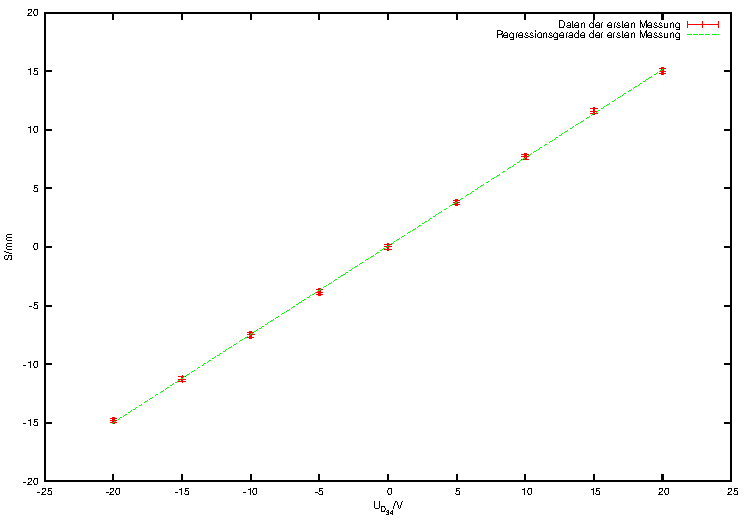
\includegraphics[scale = 1]{y_1.pdf}
  	\caption[Plot der Auslenkung in Abhängigkeit der Ablenkungsspannung, bei 1130V Beschleunigungsspannung]{Plot der Auslenkung in Abhängigkeit der Ablenkungsspannung, bei 1130V Beschleunigungsspannung}
  \label{fig:x_1}
\end{figure}



\newpage

Für eine Beschleunigungsspannung von 1150V ergab sich die Regressionsgerade mit f(x)=$0,776 (\pm 0,007) x  + 0,27 (\pm 0,09)$, mit einem $\chi^2$ von 1,64226.

\begin{figure}[htbp] 
  \centering
    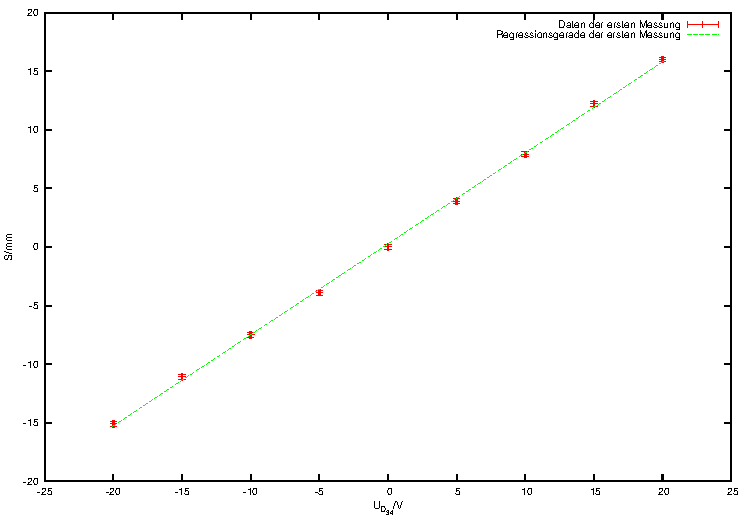
\includegraphics[scale = 1]{y_2.pdf}
  	\caption[Plot der Auslenkung in Abhängigkeit der Ablenkungsspannung, bei 1150V Beschleunigungsspannung]{Plot der Auslenkung in Abhängigkeit der Ablenkungsspannung, bei 1150V Beschleunigungsspannung}
  \label{fig:x_1}
\end{figure}


\newpage

Für eine Beschleunigungsspannung von 1325V ergab sich die Regressionsgerade mit f(x)=$0,658 (\pm 0,007) x  +0,14 (\pm 0,09)$, mit einem $\chi^2$ von 1.76032.

\begin{figure}[htbp] 
  \centering
    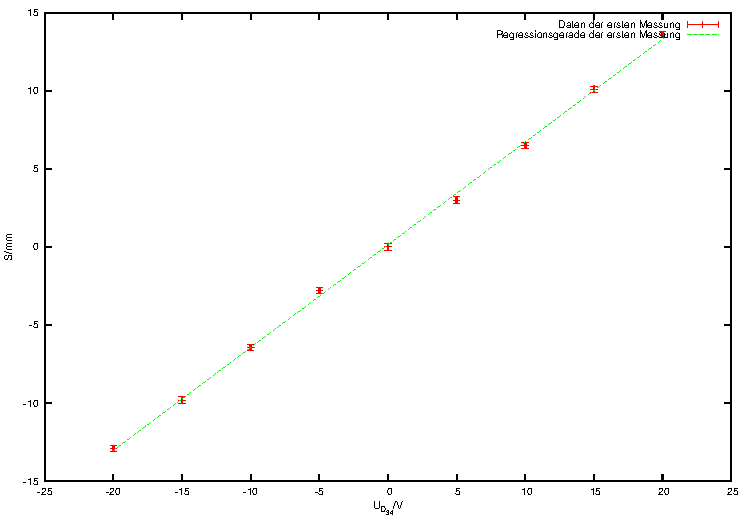
\includegraphics[scale = 1]{y_3.pdf}
  	\caption[Plot der Auslenkung in Abhängigkeit der Ablenkungsspannung, bei 1325V Beschleunigungsspannung]{Plot der Auslenkung in Abhängigkeit der Ablenkungsspannung, bei 1325V Beschleunigungsspannung}
  \label{fig:x_1}
\end{figure}

Für U$_\text{B} \cdot \text{k}$ ergab sich der Mittelwert 335 $(\pm 11)$ mm für die X-Achsenauslenkung und ein Wert von 872	$(\pm 21)$ mm Y-Achsenauslenkung (siehe Gleichung \ref{eqn:mittel} und Gleichung \ref{eqn:mittel_sigma} für den Fehler).
Daraus ergeben sich mit Gleichung \ref{eqn:Plattenabstand} und Gleichung \ref{eqn:Plattenabstand_sigma} für den Fehler die Abstände der Platten jeweils mit 3,9 $(\pm 0,3)$ mm und 2,3	$(\pm 0,2)$, der gemessene Wert liegt zwischen 2-5 mm, aufgrund der Biegung der Plättchen.

Die Messung wurde durch mehrere Faktoren beeinflusst. Dazu gehören das Erdmagnetfeld, unsere eigenen EM-Felder, die EM-Felder, die von den Geräten (Computer, Netzgeräte,...) ausgesendet wurden, als auch statische Aufladungen.
\newpage
\subsection{magnetisches Feld}

Bei der Untersuchung der Abhängigkeit zwischen der Auslenkung und der Stärke des Magnetfeldes (hier ist das Magnetfeld abhängig von der Spulenspannung U$_\text{S}$) ergaben sich die folgen den Plots.\\
Für eine Beschleunigungsspannung von 1100V ergab sich die Regressionsgerade mit f(x)=$6,5 (\pm 0,2) x  - 0,02 (\pm 0,25)$, mit einem $\chi^2$ von 0,65833.

\begin{figure}[htbp] 
  \centering
    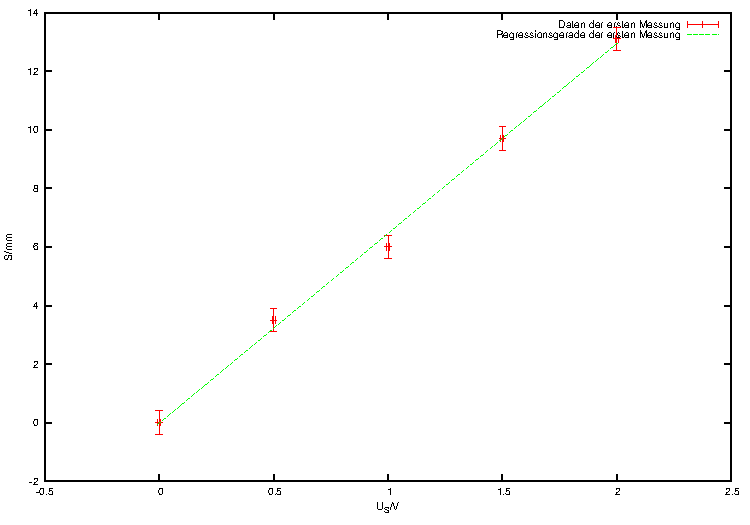
\includegraphics[scale = 1]{b_1.pdf}
  	\caption[Plot der Auslenkung in Abhängigkeit der Spulenspannung, bei 1100V Beschleunigungsspannung]{Plot der Auslenkung in Abhängigkeit der Spulenspannung, bei 1100V Beschleunigungsspannung}
  \label{fig:x_1}
\end{figure}

\newpage

Für eine Beschleunigungsspannung von 1180V ergab sich die Regressionsgerade mit f(x)=$5,5 (\pm 0,2) x  - 0,2 (\pm 0,4)$, mit einem $\chi^2$ von 1,375.

\begin{figure}[htbp] 
  \centering
    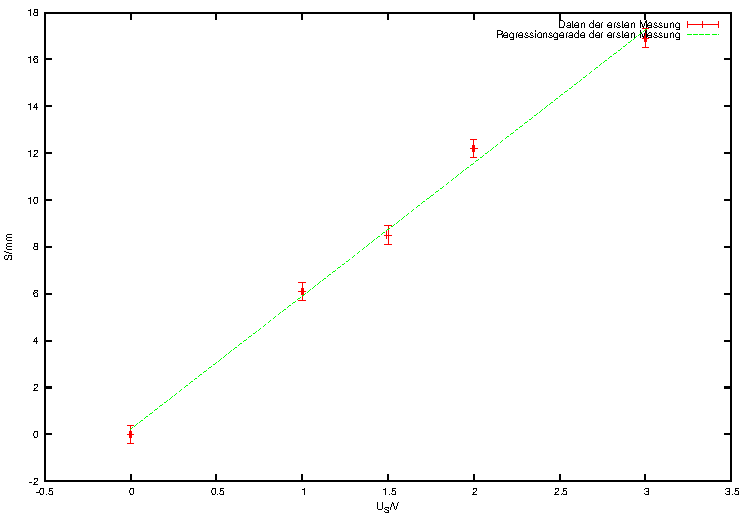
\includegraphics[scale = 1]{b_2.pdf}
  	\caption[Plot der Auslenkung in Abhängigkeit der Spulenspannung, bei 1180V Beschleunigungsspannung]{Plot der Auslenkung in Abhängigkeit der Spulenspannung, bei 1180V Beschleunigungsspannung}
  \label{fig:x_1}
\end{figure}
\newpage
Für eine Beschleunigungsspannung von 350V ergab sich die Regressionsgerade mit f(x)=$12,6 (\pm 0,6) x  - 0,2 (\pm 0,4)$, mit einem $\chi^2$ von 1.30115.

\begin{figure}[htbp] 
  \centering
    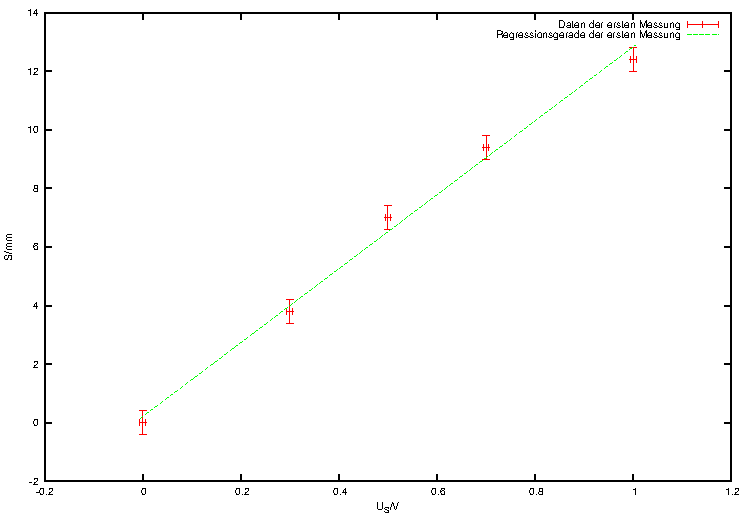
\includegraphics[scale = 1]{b_3.pdf}
  	\caption[Plot der Auslenkung in Abhängigkeit der Spulenspannung, bei 350V Beschleunigungsspannung]{Plot der Auslenkung in Abhängigkeit der Spulenspannung, bei 350V Beschleunigungsspannung}
  \label{fig:x_1}
\end{figure}

Für $k_\text{s} \cdot \sqrt{U_\text{B}}$ (vgl. Gleichung \ref{eqn:AuslenkungSpulenspannung} und Gleichung \ref{eqn:AuslenkungSpulenspannung_sigma} für den Fehler)  ergab sich bei einer Spannung von 1100V ein Wert von 223 $(\pm 6)$ $\frac{\text{mm}}{\sqrt{\text{V}}}$, bei 1180V ein Wert von 189 $(\pm 7)$ $\frac{\text{mm}}{\sqrt{\text{V}}}$ und ein Wert von 236 $(\pm 12)$ $\frac{\text{mm}}{\sqrt{\text{V}}}$ für eine Spannung von 350V. Der erste und der letzte Wert liegen innerhalb des Sigma zwei Intervalls der zweite Wert jedoch liegt sehr weit weg von den anderen beiden. Erwartet wurde, dass die drei Werte im Idealfall gleich sind.
Die Messung wurde durch mehrere Faktoren beeinflusst. Dazu gehören das Erdmagnetfeld, unsere eigenen EM-Felder, die EM-Felder, die von den Geräten (Computer, Netzgeräte,...) ausgesendet wurden, als auch statische Aufladungen.

\subsection{Erdmagnetfeld}
Bei der Bestimmung des Erdmagnetfeldes nach Gleichung \ref{eqn:bfeld} und der Fehler nach Gleichung \ref{eqn:bfeld_sigma} ergab sich ein Wert von 7,4E-005 $(\pm 1E-005)$ T, der Literaturwert liegt bei 4,8E-005 T.

\newpage
\section{Diskussion}

Im der ersten Aufgabe des Versuchsteils (a)
war es schwierig die Abstände der Ablenkplatten 1 und 2 sowie der Ablenkplatten 3 und 4 (d$_{12}$ und d$_{34}$) zu bestimmen, da der zu vermessende Bereich  durch lackiertes Glas verdeckt war.\\
Während der 6 Messungen mit verschiedenen Ablenkspannungen gab es keine Probleme, wobei auffiel, dass die linearen Fits bei zu großen als auch bei sehr kleinen Beschleunigungsspannungen schlechter wurden.
Dies liegt einerseits daran, dass die gemessene Auslenkung bei großer Beschleunigungsspannung insgesamt kleiner war, sodass die Messfehler einen größeren Anteil an den Messwerten hatten, und andererseits an dem linearen Zusammenhang zwischen Auslenkung und Ablenkspannung, der nur für kleine Winkel $\theta$ gilt ($L \gg S$).
Ebenso fällt auf, dass die Messungen in X-Achsenrichtung im Vergleich zu den Messungen in Y-Achsenrichtung besser zu dem Fit einer Geraden passen. Der Unterschied begründet sich einerseits durch die Ausrichtung des Erdmagnetfeldes, als auch dadurch, dass wir bei diesen Messungen mehrmals das Millimeterpapier berührt haben, und sich der Leuchtpunkt leicht verschoben hat.
An Formel \ref{eqn:Plattenabstand} sieht man leicht, dass das Produkt $U_B \cdot k$ konstant sein sollte, was sich auch aus den Messungen ergab.
Für den Plattenabstand nach Formel \ref{eqn:Plattenabstand} ergab sich in X-Richtung ein größerer Wert als in Y-Richtung, wobei beide Werte inerhalb der in der Versuchsbeschreibung angegebenen 2-5 mm lagen.\\
Für den Aufgabenteil (b) mussten wir die Spulenspannung variieren und sie gegen die Auslenkung auftragen und linear fitten.
Während des Versuches fiel uns auf, dass der Leuchtpunkt sich während der Messungen etwas verschob, wenn man das Millimeterpapier berührte. Der Elektronenstrahl konnte bei dieser Messung auch nur in eine Richtung ausgelenkt werden, sodass sich der Leuchtpunkt auf dem Schirm mit dem Abstand zur Mitte verformte. Deshalb haben wir doppelte Ablesefehler angenommen.
Es ergaben sich wie erwartet (Formel \ref{eqn:AuslenkungSpulenspannung}) näheungsweise Ursprungsgeraden.
Für $k_s \cdot sqrt{U_B}$ erwarten wir nach Formel \ref{eqn:AuslenkungSpulenspannung} eine Konstante. Unsere gemessenen Werte für 1100 und 350 V Beschleunigungsspannung liegen im Vergleich zum dritten Wert noch innerhalb des Sigma zwei Intervalls, wobei der Wert für 1180 V deutlich von den anderen abweicht.
Dies unterstreicht die im Vergleich zu Aufgabenteil (a) angesprochenen Schwierigkeiten bei der Messung, sowie zusätzliche Probleme bei der Fokussierung des Lichtpunktes auf dem Schirm.
Wie auch bei den Messungen in Aufgabenteil (a) kommt hinzu, dass äußere Felder Einfluß auf unsere Messungen hatten.
Insgesamt waren die Abstände in Aufgabenteil (b) schwieriger zu bestimmen als in (a).\\
Im letzten Aufgabenteil sollten wir das Erdmagnetfeld ausmessen. Obwohl der Punkt, an dem die Auslenkung verschwand, sowie der Punkt der Maximalen Auslenkung schnell gefunden war, ist mit größeren Messfehlern zu rechnen, da die Oszillographenröhre manuell gekippt werden musste und das Anzeichnen der Auslenkung dadurch schwieriger verlief (im Fall minimaler Auslenkung ist das Magnetfeld der Erde Parallel zum Elektronenstrahl). Wir mussten deshalb bei der Messung unsere Fehler größer wählen als in den Aufgaben davor. Trotzdem ist der Literaturwert von unserer Messung mehr als  zwei Sigma entfernt. Das liegt daran, dass unsere Messwerte nicht nur bei der Vermessung der Auslenkung, sondern auch bei der Messung des Abstandes vom Schrim zur Anode, welcher an einer anderen Oszillographenröhre abgeschätzt werden musste, sehr ungenau waren.
Der Abstand vom Schirm zur Anode geht zu ungunsten der Messgenauigkeit sogar quadratisch in die Berechnung des B-Feldes ein. Die letzte Messung wurde, da die Strecke, auf der der Elektronenstrahl abgelenkt wurde, länger war als in den Aufgaben davor, stärker durch äußere Einflüsse verfälscht.\\
Zusammenfassend wurde in den meisten Fällen der erwartete Zusammenhang bestätigt. Genaue Messwerte konnten meistens bedingt durch Komplikationen bei den Messungen nicht erreicht werden.
 
 %Werte stimmen mit den Formeln überein/nicht überein

\end{document}

